\chapter{Sistemas de entonaci\'on} \label{sistemasent}
La catalogaci\'on de distintos tipos de enunciados seg\'un la entonaci\'on, data de Tom\'as Navarro que define varias categor\'ias:


\begin{enumerate}
\item Entonaci\'on enunciativa: aseveraciones, enumeraciones, locuci\'on.
\item Interrogativa: preguntas aboslutas, aseverativas, pronominales, alternativas, etc. 
\item Volitiva: mandato, invitaci\'on, s\'uplica, cortes\'ia.
\item Emocional: afectaci\'on, aprobatoria, circunfleja.
\end{enumerate}


 Define 5 tonemas que son 5 tonos diferentes de la inflexi\'on final de la entonaci\'on enunciativa: cadencia, anticadencia, semicadencia, semianticadencia, suspensi\'on. A los contornos entonativos de la lengua les llama \emph{sintonema} \cite{ruiz2014entonacion}.


Hist\'oricamente, diferentes han sido los enfoques para estudiar estos llamados sintonemas. Uno de ellos es la teor\'ia m\'etrico autosegmental y otro la metodolog\'ia de Garc\'ia River\'on~(1996) \cite{garcia1996aspectos1,garcia1996aspectos2}.

\begin{comment}

 y a los patrones de la curva mel\'odica le llama sintonema. Considera 4 tipos de entonacion: l\'ogica, volitiva, emocional~(considerada la m\'as compleja de todas) e idiom\'atica \cite{ruiz2014entonacion}.



leerme conclusiones del libro
proyecto AMPER
contornos melodicos
oposiciones. q son
continuum

el entonema menos reconocido fue ve-3a

atlas linguistico de cuba
sistema entonativo
dramaturgia verbal
geografia linguistica
deseo de enseiiar un modo de hacer, ya comprobado, de la entonolog[a1 


Los estudios en el campo de la entonaci\'on como se ha dicho, en esa \'epoca~(1996), eran escasos. Solo se llegaba al acuerdo de que en verdad el fen\'omeno de la entonaci\'on era al algo dif\'icil de tratar \cite{garcia1996aspectos1}\cite{garcia2005estudio}. Se esperaba conseguir la esquematizaci\'on y formalizaci\'on de resultados en esta rama para la unidad de todos los profesionaes en sus investigaciones. No exist\'ia un sistema entonativo definido y reconocido de la entonaci\'on para el habla hispana y mucho menos para Cuba\cite{garcia1996aspectos1}.



Este libro no es, pues, stricto sensu, un manual de entonaci6n espanola en el que se recojan de manera detallada y mas 0 menos sene ilia para el estudiante universitario todas las teorras. enfoques y conocimientos actuales de esta rama del saber. Tampoco es el manual de aplicaci6n practica de los resullados de Ia invesligaci6n que podrfa allanar el camino a1 profesor de locuci6n, de lectura 0 de espanol como lengua extranjera. Estos dos tipos de manu ales seran una consecuencia 16gica de las notas iniciales que hoy se escriben
\end{comment}

\section{Modelo M\'etrico Autosegmental} \label{autosegmental}
Al comienzo de esta investigaci\'on, cuando el conocimiento sobre el estado del arte del problema era casi nulo, fue muy sugerido el an\'alisis de un modo de anotaci\'on de la entonaci\'on particular: la \emph{teoría métrico-autosegmental}.


El modelo Métrico-Autosegmental~(AM, por sus siglas en ingl\'es) nace con la propuesta de Janet Pierrehumbert para analizar la entonaci\'on del ingl\'es en su tesis doctoral de 1980 \cite{pierrehumbert1980phonology}. Ha sido revisado  y aplicado también al japonés \cite{beckman1986intonational} y a otras lenguas en obras posteriores. 


Bajo esta teor\'ia se produce la anotaci\'on del texto por \emph{acentos tonales} y \emph{tonos de frontera} basados en los acentos graves o agudos registrados en la melod\'ia, que se representan por sus iniciales en ingl\'es como un tono $L = bajo$ o $H = alto$ respectivamente. Un tono $H$ se traduce como una elevaci\'on en el movimiento de la \emph{F0} y un tono $L$, como una depresi\'on. Un acento tonal es un tono o secuencia de tonos fonológicamente asociado con una sílaba acentuada, mientras que un tono de juntura o de frontera se asocia fonológicamente con el límite de una frase . La recontrucci\'on del movimiento de la \emph{F0} se produce por la interpolaci\'on de todos los eventos tonales especificados en la transcripci\'on.


Al pronunciar una palabra aislada sin ning\'un \'enfasis especial, a la s\'ilaba t\'onica se le asocia un tono H*, donde * se utiliza para indicar que este tono se le asocia a la s\'ilaba acentuada\footnote{Cabe adjuntar, que los monosílabos como preposiciones y artículos determinados, son palabras que normalmente se pronuncian sin acento dentro de la frase.}. En la figura \ref{numero} se observa c\'omo la elevaci\'on en la curva mel\'odica var\'ia seg\'un el cambio de s\'ilaba acentuada para las palabras \emph{n\'umero}, \emph{numero} y \emph{numer\'o}. Pero esencialmente, como explica Hualde \cite{hualde2003modelo}:



\begin{quote}
 ``{La s\'ilaba t\'onica sirve, pues, de punto de “\emph{anclaje}” para ciertos eventos tonales que contribuyen a dar prominencia a esta s\'ilaba sobre las otras de la palabra, pero el tipo de contorno tonal que se asocia con la s\'ilaba acentuada depende del tipo de enunciado y de la posici\'on y relevancia pragm\'atica de la palabra dentro del mismo.}''
\end{quote}

Algo similar sucede con los tonos de frontera. De manera general a las oraciones declarativas se les asocian tonos de frontera L\% y a las interrogativas, H\%.


Aunque los acentos tonales est\'an ligados a la s\'ilaba acentuada, a la hora de transcribir una frase completa no se tienen en cuenta los acentos tonales de las s\'ilabas de todas las palabras, sino solo de aquellas que tienen prominencia  \cite{pierrehumbert1980phonology}. Por ejemplo, se ha registrado en el portugu\'es europeo que solo la primera y la \'ultima palabra reciben acento tonal en oraciones declarativas neutras \cite{hualde2003modelo}.

\begin{figure}
\begin{center}
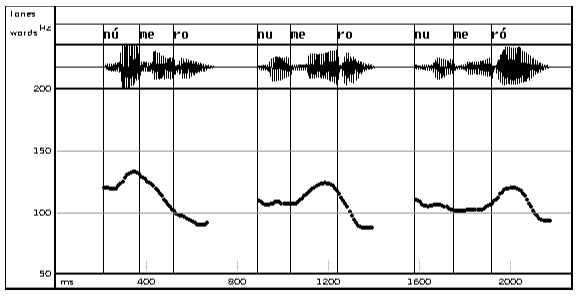
\includegraphics[width= 0.8\columnwidth]{Graphics/numero}
\caption{Pico en la t\'onica. Tomado de \cite[p.4]{hualde2003modelo}}
\label{numero}
\end{center}
\end{figure}




 Este modo de an\'alisis var\'ia de lengua a lengua tamb\'ien porque en algunas la melod\'ia tiene valor l\'exico: las llamadas lenguas tonales, como el mandar\'in. Para este tipo de lenguas se discute si es suficiente la definici\'on de solo tono alto y bajo ~($H$ y $L$). En las intonacionales, como el inglés o el español, la entonaci\'on no altera el significado de la palabra sino su valor pragm\'atico. En otros idiomas, como el sueco, la entonaci\'on tiene en parte funci\'on pragm\'atica y en parte, l\'exica \cite{hualde2003modelo}.

\subsection{Acentos tonales}
A la hora de transcribir un enunciado con el modelo AM lo primero que se debe conocer es la lengua. Para cada una se define un conjuto de acentos tonales espec\'ifico. En principio el sistema considera los siguientes acentos monotonales y bitonales:

\begin{comment}
En algunos idiomas se define un único acento tonal, por ejemplo para el japon\'es de Tokio solo existe H*+L. Para el inglés se ha propuesto un inventario con al menos 5 acentos tonales diferentes. 
\end{comment}

\begin{description} \label{tonos}
\item[H*] Pico en la tónica.
\item[L*] Valle en la tónica. 
Ejemplo: \emph{¿Me callo?} Se denotaría como L* H\% .El contorno entonativo en la s\'ilaba tónica “ca” recibe tono bajo por la interrogación y un ascenso al final de la frase.
\item[L+H*] Pico en la tónica precedido por un valle (subida de la pretónica a la tónica).
\item[L*+H] Valle en la tónica seguido por un pico (subida de la tónica a la postónica).
Ejemplo: \emph{Susana y Lucas se van ma\~nana.} (L*+H  L*+H  L+H*). Este tipo de acento es el que se observa en el espa\~nol en las palabras intermedias en las oraciones declarativas neutras sin \'enfasis especial en ninguna palabra. 
\item[H+L*] Valle en la tónica precedido por un pico (bajada de la pretónica a la tónica).
Ejemplo: \emph{Llegarán  ma\~nana.} (L*+H  H+L*  L\%).
\item[H*+L] Pico en la tónica seguido por un valle (bajada desde la tónica).
\end{description}



Con el conjunto de elementos contrastivos  definido, se detecta cada una de las s\'ilabas con acento l\'exico, solo las m\'as prominentes como se ha dicho antes, y se les asocia un acento tonal. Aunque lucen atractivas estas notaciones, es importante destacar lo confusa que resulta muchas veces y hasta entre los propios expertos, por ejemplo, al anotar un segmento espec\'ifico es debatible si ubicar un pico en la t\'onica o en la post\'onica \cite[p.72]{pierrehumbert1980phonology}.



\subsection{Tonos de frontera}

En el AM existen dos tipos de frases prosódicas: la frase entonativa y la frase intermedia. Una frase entonativa consiste en una o más frases intermedias. Al final de ambos tipos de frase podemos tener un tono de frontera.
Los tonos de frontera de frase entonativa se indican como L\%, H\%. Los tonos que marcan el final de una frase intermedia se señalan como L-, H-.

Ejemplo: \emph{¿Quieres ir a tomar helado o salir a caminar?} (H- H\%)

Esta frase entonativa contendría dos frases intermedias: “quieres ir a tomar helado” y “o salir a caminar”.



Se consideran los siguientes tonos de frontera:

\begin{description}
\item[L-L \%] Descenso final (final de oraciones declarativas).
\item[L-H\%] Descenso incompleto con subida de continuaci\'on al final.
\item[H-L\%] Suspensi\'on.
\item[H-H\%] Subida final (final de la interrogativa).
\end{description}


\begin{comment}
Se ha hablado tambi\'en de la necesidad de incluir acentos para los inicios de frase. Por ejemplo en espa\~nol las oraciones interrogativas tienen un comienzo relativamente m\'as alto que las declarativas.
\end{comment}




\subsection{Modelo ToBI}   \label{tobi}
En 1992 \cite{silverman1992tobi}, por el acuerdo entre varios especialistas y su intenci\'on de hacer una adaptaci\'on al ingl\'es del modelo AM nace el sistema ToBI~(TOnes and Break Indices). Este trata de aliviar los puntos flacos de la teor\'ia precedente\footnote{Existen muchos enfoques de an\'alisis diferentes, basta comparar una transcripci\'on con Tobi y otra con Todi ~(adaptaci\'on al holand\'es de AM) para ver lo mucho que distan a\'un cuando los contornos entonativos del ingl\'es y el holand\'es coinciden casi completamente \cite[p.23]{hualde2003modelo}.} y una de las modificaciones m\'as importantes que incluye es que permite la demarcaci\'on entre frases y palabras con la inclusi\'on de \'indices. Considera los mismos acentos tonales planteados inicialmente por AM excepto H*+L \cite{silverman1992tobi}. Se han implementado algoritmos para la anotaci\'on autom\'atica con TOBI, espec\'ificamente se puede hacer referencia a Autobi de 2010 \cite{rosenberg2010autobi}\footnote{\url{https://github.com/AndrewRosenberg/AuToBI}}.


\section{Sistema entonativo de Garc\'ia River\'on}
Similar al concepto de sintonema de Navarro, nace el de \emph{entonema}, definido por Garc\'ia River\'on como \cite{raquel2018interrogativa}:


\begin{quote}
``(...) la unidad entonativa formada por un haz de rasgos distintivos que se ordena en un eje paradigm\'atico, se realiza en un eje sintagm\'atico y cumple funciones comunicativas espec\'ificas en los actos del habla. Un cambio de \emph{entonema} puede ocasionar una ruptura de la cadena comunicativa en el texto.''
\end{quote}

La anotaci\'on por entonemas constituye un m\'etodo de transcripci\'on pros\'odica diferente: mientras que con ToBI la curva mel\'odica se reconstruye por los acentos tonales y tonos de frontera, cada entonema ya denota un comportamiento particular de la misma. A los segmentos de voz que para AM constityen frases intermedias es a los que se les asocia un tonema espec\'ifico.

Para el espa\~nol de Cuba\footnote{Espec\'ificamente el espa\~nol hablado en la capital, Ciudad de La Habana.}, la prestigiosa enton\'ologa Raquel Mar\'ia Garc\'ia River\'on ha estructurado y definido un \emph{sistema entonativo} representado por 18 entonemas principales:

\begin{description}
\item[E-1:]  Enunciaci\'on neutral. Es encontrado frecuentemente en las respuestas y en los segmentos de conclusi\'on.  
\item[VE-1a:]  Advertencia.
\item[ VE-1b:] Aclaraci\'on, evidencia. 
\item[ VE-1c:] Petici\'on marcada por un sentimiento de ruego. 
\item[ E-2:] Pregunta con alto grado de desconocimiento con respuesta argumentativa donde todos los elementos desconocidos son igualmente probables. Se considera la gran similitud que presenta con la enunciaci\'on neutral ~\cite[p.95]{garcia1996aspectos1}.
\item[ VE-2a:] Interrogaci\'on enf\'atica, con matiz categ\'orico.
\item[ E-3:] Interrogaci\'on con alto grado de desconocimiento con respuesta afirmativa o negativa.  Interrogativa absoluta.
\item[ VE-3a:] Preguntas con asombro o extrañeza. Expresan bajo grado de desconocimiento. Presentan similitud con algunas exclamaciones descritas por Antonio Quilis\footnote{Director del Laboratorio de Fon\'etica Experimental del Consejo Superior de Investigaciones Cient\'ificas de Madrid.} ~\cite[p.97, nota 13]{garcia1996aspectos1}.
\item[ VE-3b:] Interrogaci\'on de comprobaci\'on con baj\'isimo grado de desconocimiento. Corroboraci\'on, suposici\'on. Se encuentra muy cercano a la enunciaci\'on ~\cite[p.99]{garcia1996aspectos1}.
\item[ E-4:] Interrogaci\'on cuya inc\'ognita se expresa anteriormente en el di\'alogo o en el contexto. Se introducen con una \emph{Y} inicial.
\item[ VE-4a:] Interrogaci\'on inconclusa. 
\item[ E-5:] Delimitador de no conclusi\'on. Se plantea su gran similaridad con la curva de la interrogaci\'on absoluta ~\cite[p.104]{garcia1996aspectos1}. 
\item[ VE-5a:] Ejemplificador con alargamiento de la \'ultima s\'ilaba. 
\item[ VE-5b:] Argumentativa de no conclusi\'on con la cl\'ausula \emph{como}. Expresa causalidad.
\item[ E-6:] Ponderaci\'on, oraci\'on valorativa. Es una curva con terminaci\'on ascendente.
\item[ VE-6a:] Ponderaci\'on descendente. Respecto al \emph{entonema 6} no introduce valor comunicativo nuevo generalmente.
\item[ E-7:] Aperlativa.
\item[ VE-7a:] Aperlativa a distancia. 
\end{description}

Las caracter\'isticas ac\'usticas de estas categor\'ias fueron reveladas con un serio experimento en el Laboratorio de Fon\'etica Experimental del \emph{Instituto Pedag\'ogico de Lenguas Extranjeras} de Mosc\'u en el a\~no 1985 \cite{garcia1996aspectos2} y bajo la l\'inea de los \emph{rasgos distintivos}.
\begin{comment}
\subsection{Oposiciones}
Se pueden encontrar formas de entonar naturales, espont\'aneas y estimuladas psico1\'ogicamente; se utilizan formas con alguna intencionalidad y aparecen tambi\'en oposiciones en las cuales el valor psicofisiol\'ogico de la sustancia entonativa es irrelevante, por lo que entran dentro del sistema ling\"u\'istico de una lengua dada. \cite{garcia1996aspectos1}.


El contorno entonativo se puede segmentar cuando se establecen oposiciones.


Asi, a modo de ejemplo, se puede sefialar que el entonema E-l, que coincide con E-S por la forma, se diferencia de este, entre otros indicadores, por la figura del segmento poslonicO. La VE-2a coincide con E·t en la fanna, pero se diferencia de este por la figura del segmento postonico y por el nivel inicial del de la curva de enlonacion. 

\end{comment}


\subsection{Rasgos distintivos}
Garc\'ia River\'on define una serie de indicadores que permiten diferenciar los entonemas y que adem\'as tienen 
relevancia en el plano de la descripci\'on ling\"u\'istica y la funci\'on comunicativa \cite[ac\'apite 2.1.1]{garcia1996aspectos2}:
\begin{enumerate}
\item La forma
\item La figura
\item La cumbre tonal
\item El tiempo voc\'alico relativo
\item El tiempo voc\'alico m\'aximo
\item La intensidad m\'axima
\item La velocidad del fundamental
\item El registro
\item El diapas\'on
\end{enumerate}

\begin{comment}
Se ha comprobado la importancia de la forma (en relacion con el papel esencial que cum pie como rasgo diferencial de varias realidades acusticas), seguida por lafigura del segmento postonico, figura del centro de entonacion, nivel final y nivel de Fa maximo.


Es fici] de darse cuenta que, segun demuestra la somera resefia que he realizado del comportamiento de algunos de estos rasgos, fa productividad de los indicadores que nos ocupan puede variar dentro de un tipo u otro de investigacion. 


 No se descarta Ia posibilidad, ademas, de que sea necesario introducir otras tipos de indicadores 
\end{comment}

A estos les llama \emph{rasgos distintivos}. La diferenciaci\'on de los tonemas a partir de esa base, se refleja en las tablas \ref{rasgos_dist1} y \ref{rasgos_dist2}. Seg\'un la enton\'ologa, el indicador que mejor delimita los tonemas es la forma de la curva mel\'odica y es el \'unico rasgo en que se diferencian VE-1a, VE-1c, VE-2a, VE-3a, VE-3b y RE-6a~(ver Tabla \ref{rasgos_forma} anexada en el documento)  \cite[p.247]{garcia1996aspectos2}. Los siguientes par\'ametros m\'as discriminantes que declara~(ver anexo \ref{productividad}), son la figura del segmento post\'onico y el nivel final ~(regsitro).


\begin{description}
\item[La forma:] se refiere al tipo de curva que describe el movimiento de la \emph{F0}. Se detectan 4 patrones principales \emph{c\'oncava}, \emph{convexa}, \emph{recta} y \emph{zigzagueante}, incluidas tambi\'en todas sus combinaciones.
\item[La figura:] es el movimiento que realiza la curva mel\'odica dentro de una secuencia de hasta 3 s\'ilabas. Se diferencian 3 tipos: \emph{descendente}, \emph{ascendente} y \emph{llana}. Garc\'ia River\'on en su estudio, toma en cuenta este par\'ametro para el \emph{centro de la entonaci\'on} y el \emph{segmento post\'onico} \cite[p.214]{garcia1996aspectos2}.
\item[El registro o nivel del tono:] se puede determinar con la relaci\'on entre la frecuencia m\'axima y la m\'inima. En sus investigaciones, Garc\'ia River\'on analiza este par\'ametro aparejado tambi\'en a las frecuencias inicial y final.
\end{description}

\begin{comment}
rasgos mas discriminantes escalafon:
- forma
- nivel final (tercer lugar)
- diapason (4to lugar)
- nivel inicial: sirve para diferenciar ve-1c
- figura

- tiempo vocalico relativo (septimo lugar)
I. t = (Σti)/n   donde: t = media aritmética del corpus  Σ ti =  sumatoria de todos los tiempos absolutos   n=cantidad de sílabas del corpus 
II. t.voc.rel. = ti                           t


- velocidad de la f0 (octavo lugar)
- intensidad maxima (tiene baja productividad pero esta asociado a los matices afectivos)
\end{comment}





\begin{figure}
\begin{center}
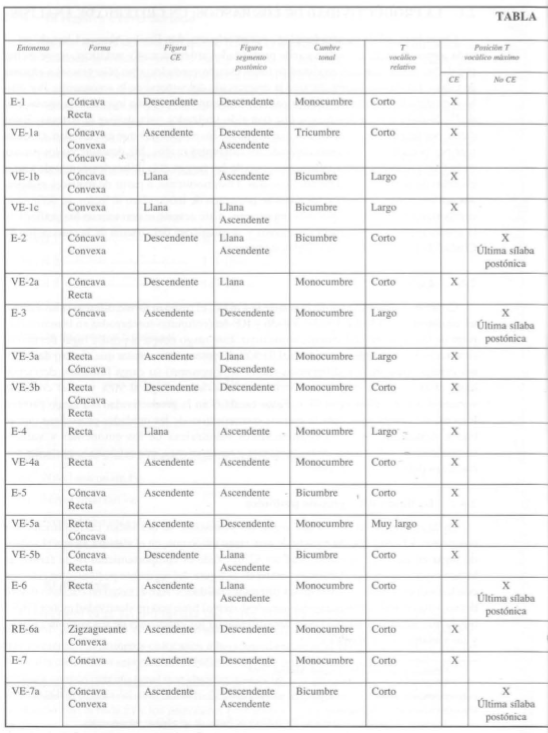
\includegraphics[width= 1\columnwidth]{Graphics/rasgos_dist1}
\caption{Rasgos distintivos por entonemas. Parte 1. Tomado de \cite[p.218]{garcia1996aspectos2}.}
\label{rasgos_dist1}
\end{center}
\end{figure}


\begin{figure}
\begin{center}
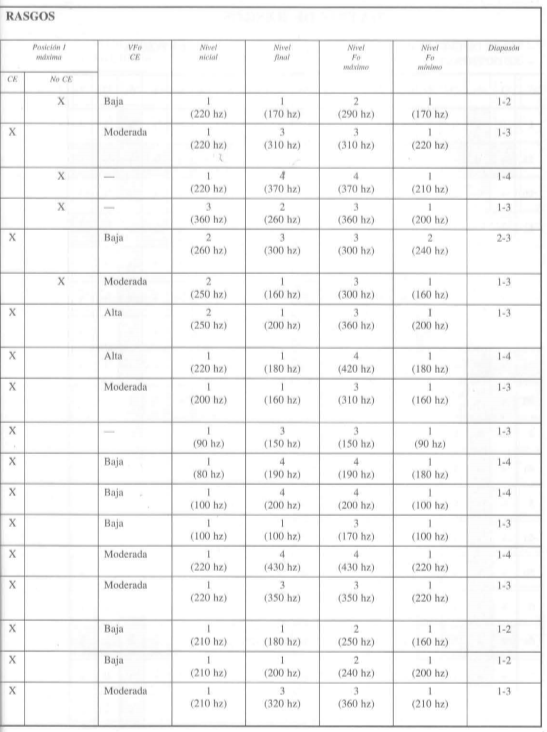
\includegraphics[width= 1\columnwidth]{Graphics/rasgos_dist2}
\caption{Rasgos distintivos por entonemas. Parte 2. Tomado de \cite[p.219]{garcia1996aspectos2}.}
\label{rasgos_dist2}
\end{center}
\end{figure}



\begin{comment}
aqui va la tablita

	\section{Comparaci\'on con sistema Tobi.}
	
	TOBI y el sistema propuesto por la doctora River\'on son ambos modelos de anotaci\'on pros\'odica solo que el primero anota por palabras y el segundo por frases. Los dos surgen para estudiar los elementos contrastivos del sistema mel\'odico~(ver tabla \ref{comparacion).
	
	\begin{table}
	\begin{center}
	\begin{tabular}{l|rr} 
	& \bf Sistema Tobi & \bf Sistema River\'on \\ \hline
	\bf Lengua    &   Ingl\'es  &    Espa\~nol de Cuba. Ciudad de La Habana   \\ 
	\bf A\~no en que se propone & 1992 & 1996 \\
	\bf M\'etodo & Transcribe por palabras cuya s\'ilaba t\'onica tiene mayor prominencia tonal y construye la curva mel\'odica con la interpolaci\'on de la combinaci\'on de los acentos tonales y tonos de frontera de dicha transcripci\'on & Anota por frases\footnote{Lo que en el sistema Tobi ser\'ia una frase intermedia} que ya tienen determinado un patr\'on de contorno mel\'odico \\
	\end{tabular}
	\caption{Comparaci\'on entre sistemas.}\label{comparacion}
	\end{center}
	\end{table}
\end{comment}


\section{Conclusiones}
Dado que ToBI y el sistema propuesto por la Dra.C. Garc\'ia River\'on son ambos modelos de anotaci\'on pros\'odica, aunque expresados en t\'erminos diferentes, se pudiera pensar que las herramientas que existen para anotar con ToBI son la soluci\'on de este problema. Esto se descarta recordando que:

\begin{enumerate}
\item La teor\'ia de Garc\'ia River\'on es antireduccionista, es decir, que apoya la idea de que no puede considerarse solo el comportamiento de la curva mel\'odica, sino tambi\'en otros rasgos como la intensidad, la duraci\'on y el timbre \cite{menendez2008estudio}.
\item Aunque algunos recursos para anotar con ToBI han sido adaptados al espa\~nol, puede que no sean efectivos con el espa\~nol de Cuba que, como bien se ha expuesto, tiene sus especificidades. Adem\'as se ha demostrado que un mismo contorno entonativo var\'ia de un hablante a otro ~(ver anexo \ref{diferencialocutor}); a\'un mayor debe ser la diferencia entre locutores de lenguas diferentes.
\end{enumerate}
